\subsection{Testbench}

De testbench is verantwoordelijk om de geschreven architecture uit te testen. De vereiste van de testbench is dat deze een klok en servoklok genereert, de servocontroller uittest in stappen van 32, de positie van de servomotor opvraagt en controleert. De servoklok mag niet gebruikt worden om het \gls{pwm} signaal te controleren.\\

\noindent
De testbench heeft zelf geen input en outputs, daarom is de entity van de testbench leeg. In de architectuur van de testbench moeten alle in- of outputsignalen  van de servocontroller aangemaakt worden, zodat deze later met het \gls{dut} kunnen verbonden worden.\\

\noindent
Verder worden ook enkele constanten aangemaakt die betrekking hebben tot de timing van de testbench. Enerzijds moeten er twee kloksignalen gegenereerd worden: De algemene klok en de servoklok. Hiertoe wordt een klokperiode (clkPeriod) en een servoklokperiode (sclkPeriod) gedefinieerd. Anderzijds worden min\_time en idle\_time gedefinieerd. Dit zijn respectievelijk de minimum duur van het \gls{pwm}signaal en de duur van het \gls{pwm}signaal in neutrale positie.\\

\noindent
Tot slot worden er nog een aantal hulpsignalen aangemaakt. EndOfSimulation is het signaal dat true wordt wanneer de simulatie klaar is. Plaats is het signaal dat gebruikt wordt om een positie aan de servocontroller door te geven. Pwm\_start en pwm\_stop zijn hulpsignalen om de timing van het \gls{pwm}signaal te controleren. 

\lstinputlisting[firstline=1,lastline=33]{tb_servo.vhd}
Na het definieren van de signalen, begint de eigenlijke architectuur van de testbench. Als eerste stap wordt het \gls{dut} op de juiste manier verbonden. Er is voor gekozen om de te testen servocontroller het adres 1 te geven.

\lstinputlisting[firstline=35,lastline=49]{tb_servo.vhd}
In een volgende stap worden de twee kloksignalen gegenereerd, die nodig zijn om de servocontroller aan te sturen.
\lstinputlisting[firstline=52,lastline=72]{tb_servo.vhd}
Het laatste proces, zal inputsignalen sturen naar de servocontroller en de output controleren. Dit proces kan in verschillende delen onderverdeelt worden.\\
\noindent
Eerst wordt de normale werking getest. Posities van 0 tot 255 worden aangelegd, in stappen van 32. Tijdens de opdracht wordt de staat van het done signaal gecontrollerd. Na een opdracht wordt er gecontroleerd of het \gls{pwm} signaal correct is. Het verwachte gedrag wordt ge\"{i}llustreerd in de volgende figuur.\\

\begin{figure}[H]
	\centering
	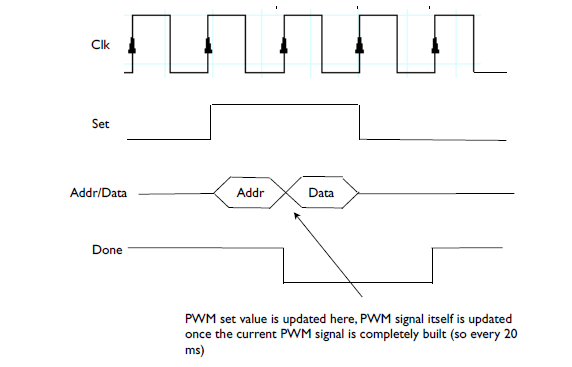
\includegraphics[width=\linewidth]{timing.png}
	\caption{Timing diagram voor de servocontroller}
\end{figure}
\noindent
De timing wordt getest met behulp van de assert/report/severity command van \gls{vhdl}. Bij een stijgende flank van de klok wordt set hoog gezet, en wordt er naar data het adres 1 gestuurd. Op de dalende flank van de klok wordt gecontroleerd of done hoog staat, anders wordt een error gerapporteerd. Na de volgende stijgende klokflank wordt de gewenste plaats naar data gestuurd. Done moet nu laag zijn, dit wordt opnieuw getest. Op de volgende stijgende flank moet set terug op laag gezet worden. Er wordt opnieuw gecontroleerd dat done laag is. Het \gls{pwm}signaal moet nog gecontroleerd worden. Pwm\_start is de timestamp van de eerstvolgende stijgende flank van het \gls{pwm}signaal, pwm\_stop is de timestamp van de eerstvolgende dalende flank. Door het verschil te berekenen tussen deze twee momenten, en te controleren met de verwachte duur van het signaal, wordt de juistheid van het \gls{pwm}signaal bepaald. Een verschil van de servoklokperiode wordt getolereerd als fout, omdat de servoklokperiode de maximale resolutie bepaald. Op dit moment wordt done voor de laatste keer getest, done moet nu hoog zijn. Dit proces wordt herhaald voor de verschillende posities.    \\
\lstinputlisting[firstline=77,lastline=121]{tb_servo.vhd}
Na de normale werking getest te hebben, moet er gecontroleerd worden of de servocontroller correct reageert op een reset. Nadat het set signaal hoog is gezet en het juiste adres is aangelegd, wordt het reset signaal korte tijd hoog gezet. Er wordt een plaats aangelegd, maar de controller mag niet naar deze plaats bewegen, in plaats daarvan moet de controller naar de neutrale (idle) positie gaan.

\lstinputlisting[firstline=123,lastline=162]{tb_servo.vhd}
Vervolgens wordt getest of de servocontroller ook luistert naar het broadcastaddress. De structuur is identiek als in de normale werking test, maar het adres is nu 255.

\lstinputlisting[firstline=166,lastline=188]{tb_servo.vhd}
Een volgende stap is het testen wat er gebeurt als de servocontroller een adres ontvangt dat niet zijn adres is, m.a.w. als de positiewijziging voor een andere servomotor bedoeld is. Het adres dat aangelegd wordt, is 2, de positie is 32\textdegree. Er wordt gecontroleerd dat de servomotor nog hetzelfde \gls{pwm}signaal geeft, nl. het signaal dat in de vorige stap (test broadcastaddress) bepaald is.

\lstinputlisting[firstline=190,lastline=226]{tb_servo.vhd}
Er kan een situatie ontstaan, waar de servocontroller wel een adres krijgt, maar geen positie. In dit geval zal set vroegtijdig laag worden. De servomotor moet dan terugvallen naar zijn reset positie. Er wordt getest wat er gebeurd als set laag wordt op de volgende stijgende klokflank: Done zal even laag worden, totdat de servocontroller beseft dat er geen verdere instructie komt. Op dat moment wordt de positie naar neutraal gebracht. Wanneer set vroeger laag wordt, zal de servocontroller bij de volgende stijgende klokflank onmiddellijk zien dat er geen verdere informatie komt en naar de neutrale positie gaan.

\lstinputlisting[firstline=228,lastline=297]{tb_servo.vhd}
Tot slot wordt er getest of de servocontroller nog steeds correct wordt wanneer er een nieuwe opdracht wordt doorgegeven onmiddellijk na de vorige. Omdat er in de vorige testen, telkens gecontroleerd werd na een verandering, kunnen er zo fouten in de reactietijd verborgen worden. Enkel de laatste positie wordt gecontroleerd.\\
\noindent
Op het einde van de simulatie wordt EndOfSim true.

\lstinputlisting[firstline=300,lastline=337]{tb_servo.vhd}